%======================================================================
\section{Experiments}
\label{sec:exp}
%======================================================================

\subsection{Setup}

We use 150 held-out questions from each of StrategyQA, MMLU-Hard, and TruthfulQA. Each condition uses five agents, three synchronous rounds, and DeepSeek-V3 as the primary backend~\cite{deepseek2024v3}. The confirmatory suite contains $450\times3=1{,}350$ question-condition records and 20,250 agent-rounds. Questions, seeds, panels, rounds, and aggregation are paired across No Mechanism, Outcome Only, and Static AEIC; only the visible offer changes. Final decisions use majority vote over the explicit third-round conclusions.

The two primary outcomes are high-effort choice rate---the share of \textsc{AEIC} and \textsc{Verify} actions---and question-level decision accuracy. We additionally report tokens per agent-round, parsing and collection integrity, and domain-level effects. Exact McNemar tests are used for paired binary outcomes and Holm-adjusted within the registered comparison family.

Figure~\ref{fig:evidence} summarizes the identification logic and the status of the evidence. The confirmatory contrast changes only the public offer within paired task units. Mechanism checks and robustness suites support interpretation of that contrast, whereas the held-out backend is treated as an external-validity boundary rather than folded into a pooled positive claim.

\begin{figure}[t]
\centering
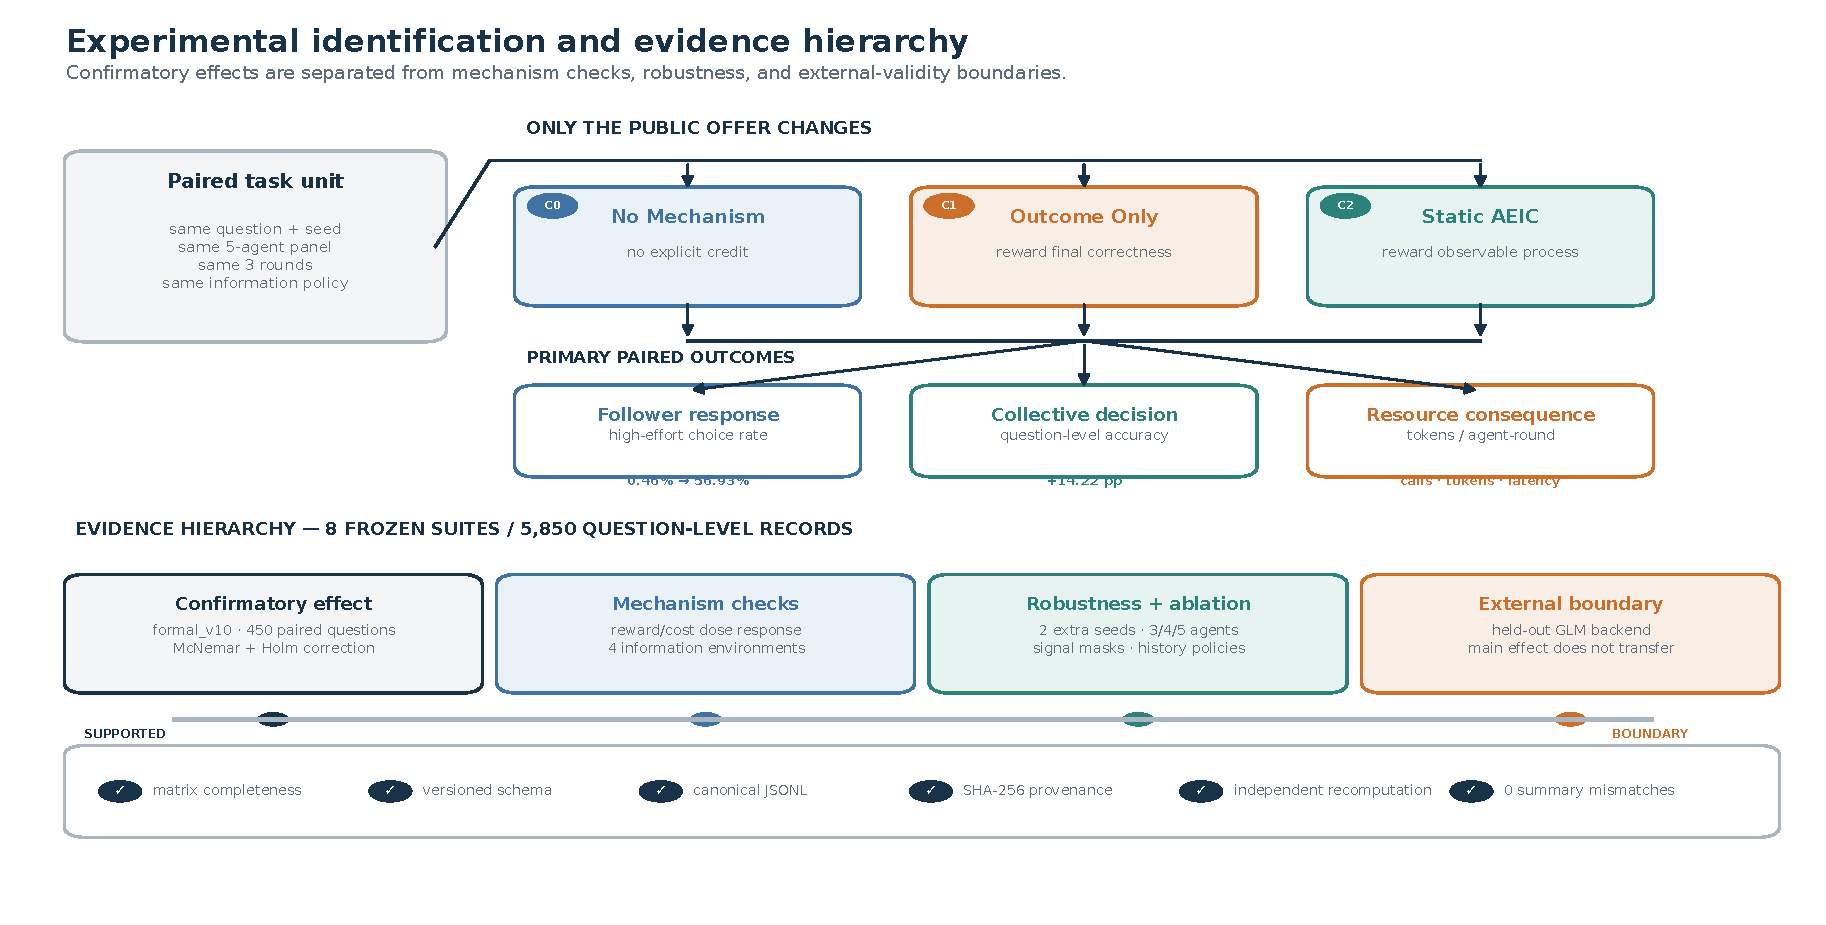
\includegraphics[width=\textwidth]{../figures/fig3_experimental_design.pdf}
\caption{Experimental identification and evidence hierarchy. Paired conditions isolate the public rule; primary outcomes measure follower response, collective accuracy, and resource use. Eight frozen suites cover confirmation, mechanism checks, robustness, ablation, and the explicit non-transfer boundary.}
\label{fig:evidence}
\end{figure}

\subsection{Confirmatory Follower-Response Test}

\begin{table}[t]
\caption{Confirmatory paired test across 450 questions. High effort is measured over 6,750 agent-rounds per rule; accuracy is measured over 450 questions.}
\label{tab:main}
\centering\small
\begin{tabular}{@{}lccc@{}}
\toprule
Rule & High effort & Accuracy & Tokens/agent-round \\
\midrule
No mechanism & 0.46\% & 68.00\% & 663.3 \\
Outcome only & 3.08\% & 67.33\% & 689.2 \\
Static AEIC & \textbf{56.93\%} & \textbf{82.22\%} & 808.8 \\
\bottomrule
\end{tabular}
\end{table}

Static AEIC changes both follower behavior and the collective decision (Table~\ref{tab:main}; Figure~\ref{fig:formal}). High-effort choice increases by 56.47 percentage points. Accuracy rises by 14.22 points, with 78 questions corrected and 14 harmed relative to No Mechanism (Holm-adjusted McNemar $p=1.23\times10^{-11}$). The additional 145.5 tokens per agent-round are consistent with the intended resource cost of more complete work.

Outcome Only is an informative control. It raises high effort by only 2.62 points and accuracy changes by $-0.67$ points (27 questions corrected, 24 harmed; $p=0.780$). Therefore, the main effect cannot be summarized as ``telling the model that a reward exists.'' What differs is whether the rule exposes a criterion the follower can satisfy through the chosen production process.

\begin{figure}[t]
\centering
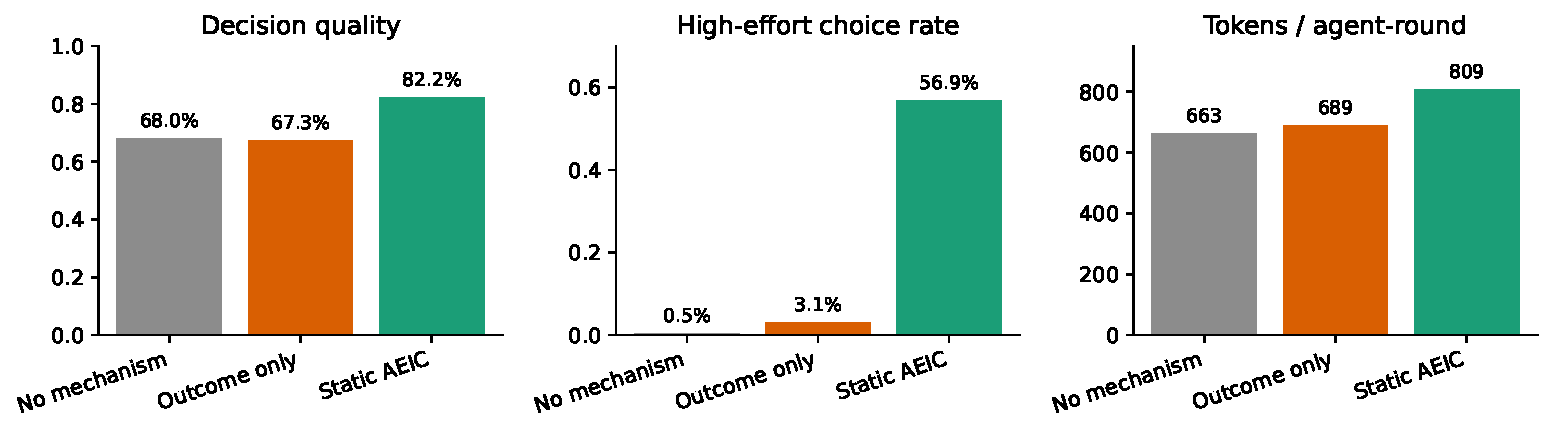
\includegraphics[width=\columnwidth]{figures/fig1_formal_mechanism.pdf}
\caption{Formal paired comparison. Static AEIC changes the declared effort action and improves final accuracy; an outcome-only reward does not improve accuracy.}
\label{fig:formal}
\end{figure}

The gain occurs in all three domains but is heterogeneous: $+4.0$ points on StrategyQA, $+20.0$ on MMLU-Hard, and $+18.7$ on TruthfulQA. The corresponding increases in high effort are 43.5, 73.7, and 52.2 points. This heterogeneity argues against interpreting the pooled effect as a task-independent constant.

\subsection{Reward--Cost Response}

For every domain, high-effort choice is monotone non-decreasing as the revealed reward scale moves from 0.05 to 0.2 to 0.5, and monotone non-increasing as the effort-cost multiplier moves from 0.5 to 1.0 to 1.5 (Figure~\ref{fig:boundary}). At the pooled frozen extremes, high effort rises from 49.42\% at reward 0.05 to 72.84\% at reward 0.5; it falls from 69.51\% at cost multiplier 0.5 to 53.78\% at 1.5. Because the middle points are same-domain development observations whereas the extremes are separately frozen, this is a directional mechanism check rather than a second confirmatory effect estimate.

\begin{figure}[t]
\centering
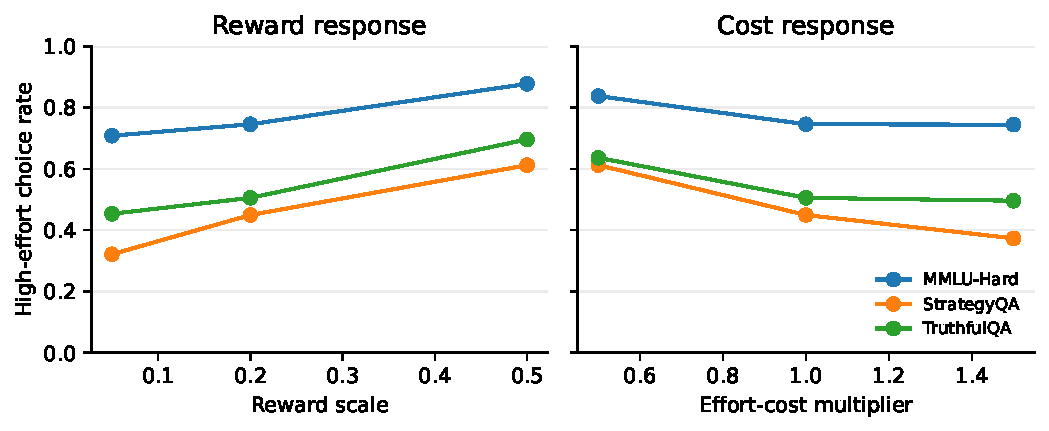
\includegraphics[width=\columnwidth]{figures/fig2_incentive_response.pdf}
\caption{Directional response to the public offer. Within every domain, effort rises with revealed reward and falls with action cost.}
\label{fig:boundary}
\end{figure}

\subsection{Controlled Information Environments}

We next vary only what peer information is available after the first round: one new evidence item, a majority stance without evidence, full reports plus copy pressure, or stance-opposing evidence. Across these four environments, Static AEIC raises pooled high effort from 0.86\% to 49.41\%. Condition-specific rates under Static AEIC range from 40.89\% (social only) to 59.33\% (copy pressure), compared with 0.44\%--1.47\% without a mechanism (Figure~\ref{fig:info}). These manipulations confirm that the report interface remains behaviorally operative under distinct information structures. They do not establish that every information intervention improves accuracy or eliminates imitation.

\begin{figure}[t]
\centering
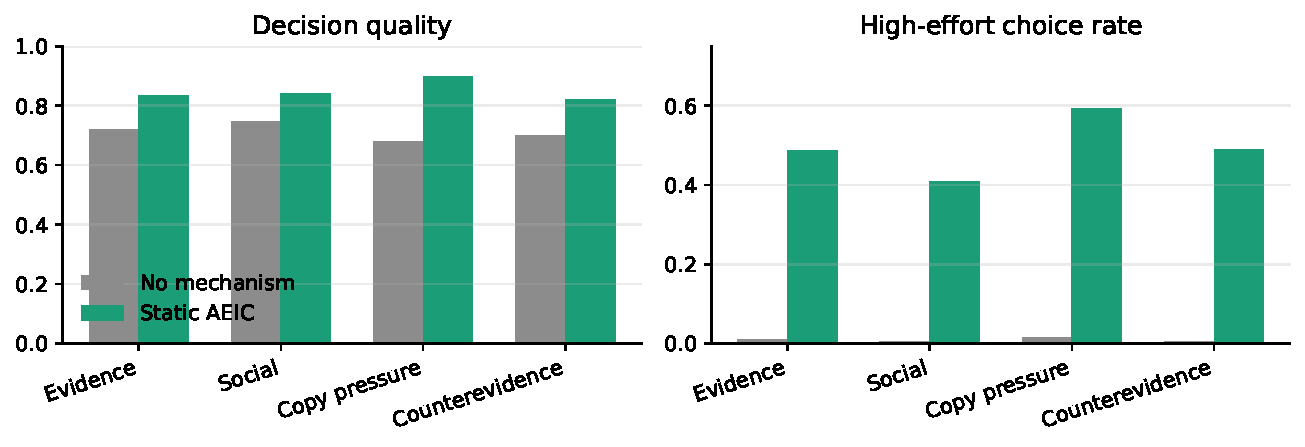
\includegraphics[width=\columnwidth]{figures/fig3_information_conditions.pdf}
\caption{High-effort actions under controlled information environments. Static AEIC shifts behavior in all four settings.}
\label{fig:info}
\end{figure}

\subsection{Robustness, Ablation, and External Validity}

Two additional seeds reproduce the main direction: Static AEIC reaches 85.67\% accuracy versus 71.00\% without a mechanism ($+14.67$ points; Holm-adjusted $p=2.40\times10^{-9}$). With three, four, and five agents, its accuracy lies between 87.33\% and 88.67\%. Signal-mask and history-policy variants are summarized in Figure~\ref{fig:robust}; they bound the current implementation but do not show that each AEIC field is individually necessary. In particular, removing a field can change how the backend interprets the entire visible contract, so these are intervention ablations rather than modular proofs.

\begin{figure}[t]
\centering
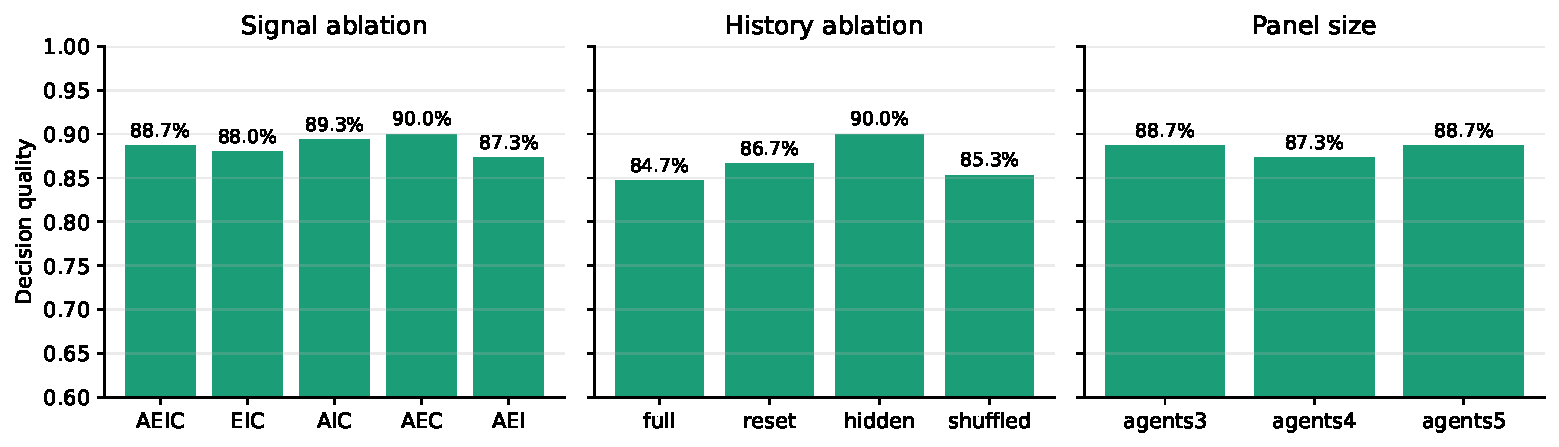
\includegraphics[width=\columnwidth]{figures/fig4_ablations_robustness.pdf}
\caption{Signal, history, seed, and panel-size robustness. Component variants are descriptive boundaries rather than isolated necessity proofs.}
\label{fig:robust}
\end{figure}

The held-out GLM backend is the strongest boundary result. Static AEIC barely changes high effort (0.58\% to 0.93\%, $p=0.134$) and yields 69.33\% accuracy versus 70.67\% without a mechanism (Holm-adjusted $p=0.791$). The same words and numerical schedule therefore do not define the same effective contract across model families. This failure is reported in the main text because it changes the scope of the contribution: AEIC-MD is an experimentally validated mechanism for the tested primary backend, not a universally calibrated incentive language.

\subsection{Integrity and Reproducibility}

Across the eight frozen suites, all 5,850 expected question-level records are present. Every suite passes schema and route validation and has an independently recomputed bundle with no summary mismatch. In the confirmatory data, API terminal failure is zero and cost logging is complete; rare parse failures are retried and remain visible in attempt logs. The manifest stores canonical hashes for each suite, preventing silent replacement of the analyzed records.
